% Created by tikzDevice version 0.12.3.1 on 2022-05-11 18:52:39
% !TEX encoding = UTF-8 Unicode
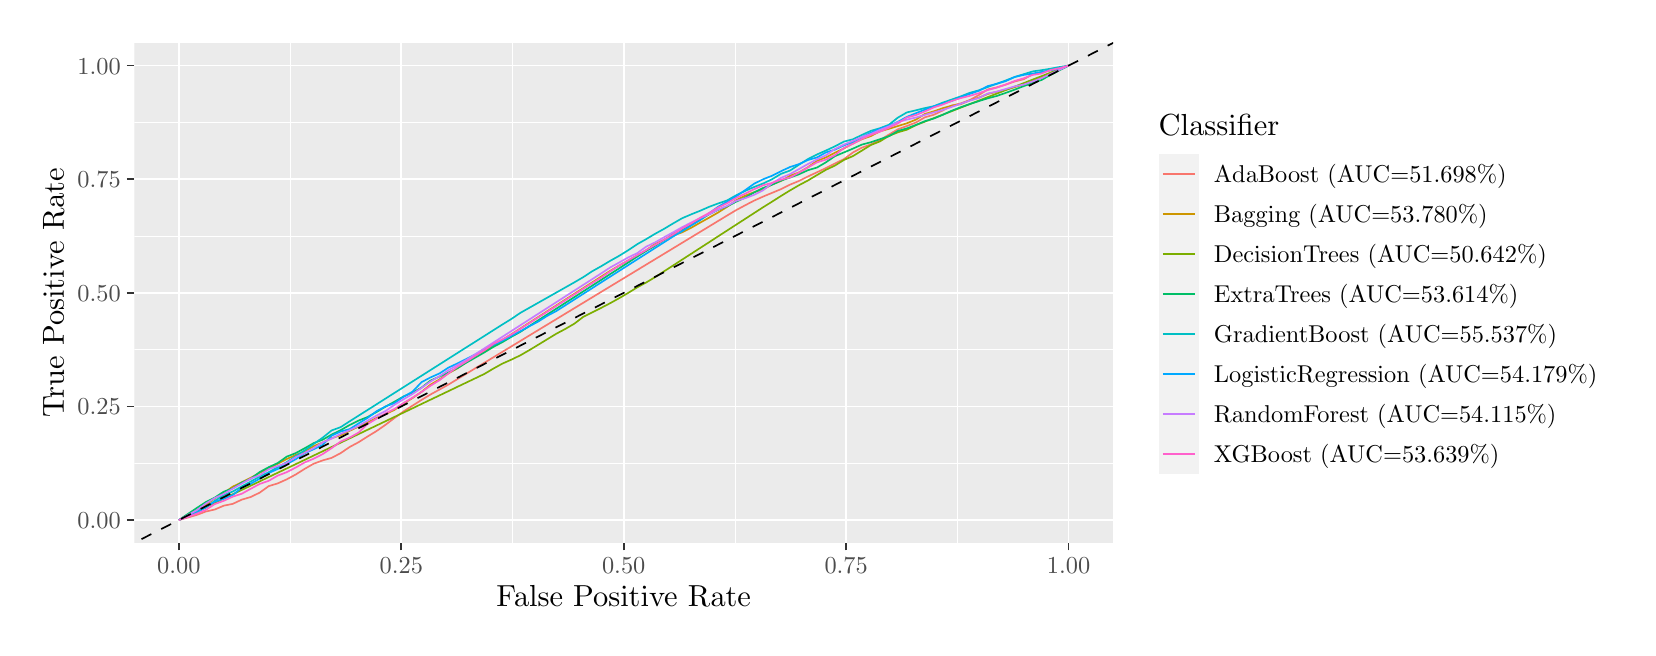
\begin{tikzpicture}[x=1pt,y=1pt]
\definecolor{fillColor}{RGB}{255,255,255}
\path[use as bounding box,fill=fillColor,fill opacity=0.00] (0,0) rectangle (578.16,216.81);
\begin{scope}
\path[clip] (  0.00,  0.00) rectangle (578.16,216.81);
\definecolor{drawColor}{RGB}{255,255,255}
\definecolor{fillColor}{RGB}{255,255,255}

\path[draw=drawColor,line width= 0.6pt,line join=round,line cap=round,fill=fillColor] (  0.00,  0.00) rectangle (578.16,216.81);
\end{scope}
\begin{scope}
\path[clip] ( 38.56, 30.69) rectangle (392.21,211.31);
\definecolor{fillColor}{gray}{0.92}

\path[fill=fillColor] ( 38.56, 30.69) rectangle (392.21,211.31);
\definecolor{drawColor}{RGB}{255,255,255}

\path[draw=drawColor,line width= 0.3pt,line join=round] ( 38.56, 59.42) --
	(392.21, 59.42);

\path[draw=drawColor,line width= 0.3pt,line join=round] ( 38.56,100.47) --
	(392.21,100.47);

\path[draw=drawColor,line width= 0.3pt,line join=round] ( 38.56,141.52) --
	(392.21,141.52);

\path[draw=drawColor,line width= 0.3pt,line join=round] ( 38.56,182.57) --
	(392.21,182.57);

\path[draw=drawColor,line width= 0.3pt,line join=round] ( 94.82, 30.69) --
	( 94.82,211.31);

\path[draw=drawColor,line width= 0.3pt,line join=round] (175.20, 30.69) --
	(175.20,211.31);

\path[draw=drawColor,line width= 0.3pt,line join=round] (255.57, 30.69) --
	(255.57,211.31);

\path[draw=drawColor,line width= 0.3pt,line join=round] (335.95, 30.69) --
	(335.95,211.31);

\path[draw=drawColor,line width= 0.6pt,line join=round] ( 38.56, 38.90) --
	(392.21, 38.90);

\path[draw=drawColor,line width= 0.6pt,line join=round] ( 38.56, 79.95) --
	(392.21, 79.95);

\path[draw=drawColor,line width= 0.6pt,line join=round] ( 38.56,121.00) --
	(392.21,121.00);

\path[draw=drawColor,line width= 0.6pt,line join=round] ( 38.56,162.05) --
	(392.21,162.05);

\path[draw=drawColor,line width= 0.6pt,line join=round] ( 38.56,203.10) --
	(392.21,203.10);

\path[draw=drawColor,line width= 0.6pt,line join=round] ( 54.63, 30.69) --
	( 54.63,211.31);

\path[draw=drawColor,line width= 0.6pt,line join=round] (135.01, 30.69) --
	(135.01,211.31);

\path[draw=drawColor,line width= 0.6pt,line join=round] (215.38, 30.69) --
	(215.38,211.31);

\path[draw=drawColor,line width= 0.6pt,line join=round] (295.76, 30.69) --
	(295.76,211.31);

\path[draw=drawColor,line width= 0.6pt,line join=round] (376.14, 30.69) --
	(376.14,211.31);
\definecolor{drawColor}{RGB}{248,118,109}

\path[draw=drawColor,line width= 0.6pt,line join=round] ( 54.63, 38.90) --
	( 57.88, 39.80) --
	( 61.13, 40.75) --
	( 64.37, 41.96) --
	( 67.62, 42.70) --
	( 70.87, 44.09) --
	( 74.12, 44.74) --
	( 77.36, 46.26) --
	( 80.61, 47.22) --
	( 83.86, 48.81) --
	( 87.11, 51.15) --
	( 90.35, 52.13) --
	( 93.60, 53.59) --
	( 96.85, 55.34) --
	(100.10, 57.39) --
	(103.34, 59.24) --
	(106.59, 60.44) --
	(109.84, 61.36) --
	(113.09, 63.07) --
	(116.33, 65.28) --
	(119.58, 67.02) --
	(122.83, 69.08) --
	(126.08, 71.06) --
	(129.32, 73.32) --
	(132.57, 75.79) --
	(135.82, 78.14) --
	(139.07, 80.23) --
	(142.31, 82.29) --
	(145.56, 84.26) --
	(148.81, 86.04) --
	(152.06, 87.85) --
	(155.30, 89.82) --
	(158.55, 91.79) --
	(161.80, 93.76) --
	(165.05, 95.73) --
	(168.29, 97.70) --
	(171.54, 99.67) --
	(174.79,101.64) --
	(178.04,103.61) --
	(181.28,105.58) --
	(184.53,107.55) --
	(187.78,109.52) --
	(191.03,111.49) --
	(194.27,113.46) --
	(197.52,115.43) --
	(200.77,117.40) --
	(204.02,119.37) --
	(207.26,121.34) --
	(210.51,123.31) --
	(213.76,125.28) --
	(217.01,127.25) --
	(220.26,129.22) --
	(223.50,131.19) --
	(226.75,133.16) --
	(230.00,135.13) --
	(233.25,137.10) --
	(236.49,139.07) --
	(239.74,141.04) --
	(242.99,143.01) --
	(246.24,144.98) --
	(249.48,146.95) --
	(252.73,148.92) --
	(255.98,150.87) --
	(259.23,152.61) --
	(262.47,154.30) --
	(265.72,155.76) --
	(268.97,157.11) --
	(272.22,158.46) --
	(275.46,160.08) --
	(278.71,161.42) --
	(281.96,163.05) --
	(285.21,164.55) --
	(288.45,166.08) --
	(291.70,167.74) --
	(294.95,169.30) --
	(298.20,171.70) --
	(301.44,173.46) --
	(304.69,174.64) --
	(307.94,176.16) --
	(311.19,178.16) --
	(314.43,180.09) --
	(317.68,181.26) --
	(320.93,182.53) --
	(324.18,184.41) --
	(327.42,185.34) --
	(330.67,186.89) --
	(333.92,188.66) --
	(337.17,189.44) --
	(340.41,190.66) --
	(343.66,192.44) --
	(346.91,194.49) --
	(350.16,195.23) --
	(353.40,196.23) --
	(356.65,197.35) --
	(359.90,198.16) --
	(363.15,199.98) --
	(366.39,200.68) --
	(369.64,201.38) --
	(372.89,202.20) --
	(376.14,203.10);
\definecolor{drawColor}{RGB}{205,150,0}

\path[draw=drawColor,line width= 0.6pt,line join=round] ( 54.63, 38.90) --
	( 57.88, 40.48) --
	( 61.13, 42.42) --
	( 64.37, 44.35) --
	( 67.62, 46.73) --
	( 70.87, 48.67) --
	( 74.12, 50.96) --
	( 77.36, 52.56) --
	( 80.61, 54.16) --
	( 83.86, 55.97) --
	( 87.11, 57.60) --
	( 90.35, 59.22) --
	( 93.60, 60.93) --
	( 96.85, 62.41) --
	(100.10, 63.64) --
	(103.34, 65.60) --
	(106.59, 66.90) --
	(109.84, 68.46) --
	(113.09, 69.53) --
	(116.33, 71.12) --
	(119.58, 72.65) --
	(122.83, 74.12) --
	(126.08, 75.81) --
	(129.32, 77.13) --
	(132.57, 78.72) --
	(135.82, 81.02) --
	(139.07, 82.97) --
	(142.31, 85.20) --
	(145.56, 87.81) --
	(148.81, 89.71) --
	(152.06, 91.93) --
	(155.30, 93.69) --
	(158.55, 95.98) --
	(161.80, 97.85) --
	(165.05, 99.78) --
	(168.29,101.86) --
	(171.54,103.95) --
	(174.79,106.03) --
	(178.04,108.11) --
	(181.28,110.20) --
	(184.53,112.28) --
	(187.78,114.36) --
	(191.03,116.45) --
	(194.27,118.53) --
	(197.52,120.62) --
	(200.77,122.70) --
	(204.02,124.78) --
	(207.26,126.87) --
	(210.51,128.95) --
	(213.76,130.86) --
	(217.01,132.69) --
	(220.26,134.50) --
	(223.50,136.41) --
	(226.75,138.67) --
	(230.00,140.14) --
	(233.25,141.78) --
	(236.49,142.84) --
	(239.74,144.49) --
	(242.99,146.35) --
	(246.24,148.16) --
	(249.48,150.01) --
	(252.73,152.05) --
	(255.98,154.46) --
	(259.23,156.08) --
	(262.47,157.36) --
	(265.72,158.34) --
	(268.97,160.13) --
	(272.22,161.42) --
	(275.46,163.29) --
	(278.71,164.51) --
	(281.96,166.39) --
	(285.21,168.67) --
	(288.45,169.92) --
	(291.70,171.63) --
	(294.95,173.16) --
	(298.20,174.96) --
	(301.44,176.50) --
	(304.69,177.64) --
	(307.94,179.35) --
	(311.19,180.25) --
	(314.43,181.26) --
	(317.68,182.25) --
	(320.93,183.56) --
	(324.18,185.62) --
	(327.42,186.57) --
	(330.67,187.73) --
	(333.92,188.63) --
	(337.17,189.17) --
	(340.41,190.54) --
	(343.66,191.50) --
	(346.91,192.84) --
	(350.16,193.62) --
	(353.40,194.38) --
	(356.65,195.31) --
	(359.90,196.31) --
	(363.15,197.52) --
	(366.39,198.73) --
	(369.64,200.28) --
	(372.89,201.71) --
	(376.14,203.10);
\definecolor{drawColor}{RGB}{124,174,0}

\path[draw=drawColor,line width= 0.6pt,line join=round] ( 54.63, 38.90) --
	( 57.88, 40.45) --
	( 61.13, 42.00) --
	( 64.37, 43.55) --
	( 67.62, 45.11) --
	( 70.87, 46.66) --
	( 74.12, 48.21) --
	( 77.36, 49.77) --
	( 80.61, 51.32) --
	( 83.86, 52.87) --
	( 87.11, 54.43) --
	( 90.35, 55.98) --
	( 93.60, 57.53) --
	( 96.85, 59.08) --
	(100.10, 60.64) --
	(103.34, 62.19) --
	(106.59, 63.74) --
	(109.84, 65.30) --
	(113.09, 66.85) --
	(116.33, 68.40) --
	(119.58, 69.95) --
	(122.83, 71.51) --
	(126.08, 73.06) --
	(129.32, 74.61) --
	(132.57, 76.17) --
	(135.82, 77.72) --
	(139.07, 79.27) --
	(142.31, 80.83) --
	(145.56, 82.38) --
	(148.81, 83.93) --
	(152.06, 85.48) --
	(155.30, 87.04) --
	(158.55, 88.59) --
	(161.80, 90.14) --
	(165.05, 91.70) --
	(168.29, 93.62) --
	(171.54, 95.42) --
	(174.79, 96.85) --
	(178.04, 98.42) --
	(181.28,100.29) --
	(184.53,102.25) --
	(187.78,104.24) --
	(191.03,106.22) --
	(194.27,107.94) --
	(197.52,109.83) --
	(200.77,112.31) --
	(204.02,113.92) --
	(207.26,115.57) --
	(210.51,117.26) --
	(213.76,119.07) --
	(217.01,120.97) --
	(220.26,122.97) --
	(223.50,124.73) --
	(226.75,126.69) --
	(230.00,128.79) --
	(233.25,130.89) --
	(236.49,132.99) --
	(239.74,135.09) --
	(242.99,137.19) --
	(246.24,139.29) --
	(249.48,141.40) --
	(252.73,143.50) --
	(255.98,145.60) --
	(259.23,147.70) --
	(262.47,149.80) --
	(265.72,151.90) --
	(268.97,153.93) --
	(272.22,156.00) --
	(275.46,157.99) --
	(278.71,159.88) --
	(281.96,161.60) --
	(285.21,163.54) --
	(288.45,165.45) --
	(291.70,166.97) --
	(294.95,169.01) --
	(298.20,170.40) --
	(301.44,172.39) --
	(304.69,174.40) --
	(307.94,175.70) --
	(311.19,177.69) --
	(314.43,178.99) --
	(317.68,179.93) --
	(320.93,181.58) --
	(324.18,182.85) --
	(327.42,184.11) --
	(330.67,185.38) --
	(333.92,186.64) --
	(337.17,187.91) --
	(340.41,189.18) --
	(343.66,190.44) --
	(346.91,191.71) --
	(350.16,192.97) --
	(353.40,194.24) --
	(356.65,195.50) --
	(359.90,196.77) --
	(363.15,198.04) --
	(366.39,199.30) --
	(369.64,200.57) --
	(372.89,201.83) --
	(376.14,203.10);
\definecolor{drawColor}{RGB}{0,190,103}

\path[draw=drawColor,line width= 0.6pt,line join=round] ( 54.63, 38.90) --
	( 57.88, 41.08) --
	( 61.13, 43.27) --
	( 64.37, 45.37) --
	( 67.62, 47.02) --
	( 70.87, 49.15) --
	( 74.12, 50.33) --
	( 77.36, 52.42) --
	( 80.61, 53.80) --
	( 83.86, 56.25) --
	( 87.11, 58.00) --
	( 90.35, 59.49) --
	( 93.60, 61.80) --
	( 96.85, 63.08) --
	(100.10, 64.84) --
	(103.34, 66.68) --
	(106.59, 67.92) --
	(109.84, 69.78) --
	(113.09, 71.36) --
	(116.33, 73.23) --
	(119.58, 74.83) --
	(122.83, 76.12) --
	(126.08, 77.94) --
	(129.32, 79.88) --
	(132.57, 81.67) --
	(135.82, 83.54) --
	(139.07, 84.95) --
	(142.31, 86.73) --
	(145.56, 89.29) --
	(148.81, 90.73) --
	(152.06, 92.20) --
	(155.30, 93.80) --
	(158.55, 95.77) --
	(161.80, 97.62) --
	(165.05, 99.48) --
	(168.29,101.46) --
	(171.54,103.17) --
	(174.79,105.10) --
	(178.04,106.89) --
	(181.28,109.01) --
	(184.53,111.10) --
	(187.78,113.18) --
	(191.03,115.27) --
	(194.27,117.35) --
	(197.52,119.44) --
	(200.77,121.52) --
	(204.02,123.61) --
	(207.26,125.69) --
	(210.51,127.78) --
	(213.76,129.86) --
	(217.01,131.95) --
	(220.26,134.08) --
	(223.50,136.12) --
	(226.75,138.02) --
	(230.00,140.11) --
	(233.25,142.25) --
	(236.49,143.89) --
	(239.74,145.74) --
	(242.99,147.44) --
	(246.24,149.35) --
	(249.48,150.97) --
	(252.73,152.23) --
	(255.98,153.90) --
	(259.23,155.37) --
	(262.47,157.25) --
	(265.72,158.88) --
	(268.97,160.04) --
	(272.22,161.54) --
	(275.46,162.63) --
	(278.71,163.83) --
	(281.96,165.31) --
	(285.21,166.26) --
	(288.45,168.16) --
	(291.70,170.38) --
	(294.95,171.73) --
	(298.20,173.10) --
	(301.44,174.56) --
	(304.69,175.42) --
	(307.94,176.52) --
	(311.19,177.57) --
	(314.43,179.48) --
	(317.68,180.41) --
	(320.93,181.64) --
	(324.18,183.02) --
	(327.42,183.98) --
	(330.67,185.32) --
	(333.92,186.81) --
	(337.17,188.07) --
	(340.41,189.20) --
	(343.66,190.25) --
	(346.91,191.27) --
	(350.16,192.12) --
	(353.40,193.24) --
	(356.65,194.42) --
	(359.90,195.68) --
	(363.15,196.82) --
	(366.39,197.92) --
	(369.64,199.79) --
	(372.89,201.42) --
	(376.14,203.10);
\definecolor{drawColor}{RGB}{0,191,196}

\path[draw=drawColor,line width= 0.6pt,line join=round] ( 54.63, 38.90) --
	( 57.88, 40.26) --
	( 61.13, 42.06) --
	( 64.37, 43.32) --
	( 67.62, 45.84) --
	( 70.87, 47.91) --
	( 74.12, 49.20) --
	( 77.36, 51.07) --
	( 80.61, 52.81) --
	( 83.86, 54.58) --
	( 87.11, 56.18) --
	( 90.35, 57.99) --
	( 93.60, 59.80) --
	( 96.85, 61.96) --
	(100.10, 64.08) --
	(103.34, 66.37) --
	(106.59, 68.66) --
	(109.84, 71.27) --
	(113.09, 72.46) --
	(116.33, 74.56) --
	(119.58, 76.62) --
	(122.83, 78.67) --
	(126.08, 80.73) --
	(129.32, 82.79) --
	(132.57, 84.85) --
	(135.82, 86.91) --
	(139.07, 88.97) --
	(142.31, 91.02) --
	(145.56, 93.08) --
	(148.81, 95.14) --
	(152.06, 97.20) --
	(155.30, 99.26) --
	(158.55,101.32) --
	(161.80,103.37) --
	(165.05,105.43) --
	(168.29,107.49) --
	(171.54,109.55) --
	(174.79,111.55) --
	(178.04,113.76) --
	(181.28,115.59) --
	(184.53,117.43) --
	(187.78,119.26) --
	(191.03,121.10) --
	(194.27,122.93) --
	(197.52,124.77) --
	(200.77,126.67) --
	(204.02,128.80) --
	(207.26,130.62) --
	(210.51,132.56) --
	(213.76,134.38) --
	(217.01,136.39) --
	(220.26,138.57) --
	(223.50,140.40) --
	(226.75,142.34) --
	(230.00,144.13) --
	(233.25,146.08) --
	(236.49,147.95) --
	(239.74,149.34) --
	(242.99,150.65) --
	(246.24,152.07) --
	(249.48,153.28) --
	(252.73,154.39) --
	(255.98,156.23) --
	(259.23,157.81) --
	(262.47,159.22) --
	(265.72,160.49) --
	(268.97,162.03) --
	(272.22,164.00) --
	(275.46,165.17) --
	(278.71,167.28) --
	(281.96,169.34) --
	(285.21,170.98) --
	(288.45,172.42) --
	(291.70,173.93) --
	(294.95,175.65) --
	(298.20,176.48) --
	(301.44,178.05) --
	(304.69,179.53) --
	(307.94,180.48) --
	(311.19,181.71) --
	(314.43,184.30) --
	(317.68,186.18) --
	(320.93,186.94) --
	(324.18,187.75) --
	(327.42,188.43) --
	(330.67,189.74) --
	(333.92,190.85) --
	(337.17,191.99) --
	(340.41,193.26) --
	(343.66,194.16) --
	(346.91,195.35) --
	(350.16,196.53) --
	(353.40,197.72) --
	(356.65,199.00) --
	(359.90,199.99) --
	(363.15,201.00) --
	(366.39,201.46) --
	(369.64,201.99) --
	(372.89,202.60) --
	(376.14,203.10);
\definecolor{drawColor}{RGB}{0,169,255}

\path[draw=drawColor,line width= 0.6pt,line join=round] ( 54.63, 38.90) --
	( 57.88, 40.22) --
	( 61.13, 41.50) --
	( 64.37, 43.63) --
	( 67.62, 45.56) --
	( 70.87, 46.55) --
	( 74.12, 47.95) --
	( 77.36, 50.56) --
	( 80.61, 52.03) --
	( 83.86, 53.83) --
	( 87.11, 55.89) --
	( 90.35, 57.32) --
	( 93.60, 59.09) --
	( 96.85, 60.85) --
	(100.10, 63.03) --
	(103.34, 64.47) --
	(106.59, 66.04) --
	(109.84, 69.38) --
	(113.09, 70.87) --
	(116.33, 71.75) --
	(119.58, 73.80) --
	(122.83, 75.81) --
	(126.08, 78.23) --
	(129.32, 79.95) --
	(132.57, 81.15) --
	(135.82, 83.45) --
	(139.07, 85.28) --
	(142.31, 88.72) --
	(145.56, 90.43) --
	(148.81, 91.87) --
	(152.06, 93.98) --
	(155.30, 95.49) --
	(158.55, 97.10) --
	(161.80, 98.76) --
	(165.05,100.61) --
	(168.29,102.19) --
	(171.54,103.68) --
	(174.79,105.40) --
	(178.04,107.11) --
	(181.28,108.91) --
	(184.53,110.63) --
	(187.78,112.69) --
	(191.03,114.41) --
	(194.27,116.48) --
	(197.52,118.56) --
	(200.77,120.63) --
	(204.02,122.70) --
	(207.26,124.78) --
	(210.51,126.85) --
	(213.76,128.92) --
	(217.01,131.00) --
	(220.26,133.07) --
	(223.50,135.14) --
	(226.75,137.21) --
	(230.00,139.29) --
	(233.25,141.36) --
	(236.49,143.26) --
	(239.74,145.30) --
	(242.99,147.24) --
	(246.24,149.75) --
	(249.48,152.09) --
	(252.73,153.91) --
	(255.98,155.84) --
	(259.23,158.08) --
	(262.47,160.40) --
	(265.72,162.02) --
	(268.97,163.30) --
	(272.22,164.95) --
	(275.46,166.45) --
	(278.71,167.51) --
	(281.96,168.99) --
	(285.21,169.91) --
	(288.45,171.74) --
	(291.70,172.73) --
	(294.95,174.27) --
	(298.20,175.51) --
	(301.44,177.22) --
	(304.69,178.85) --
	(307.94,180.27) --
	(311.19,181.36) --
	(314.43,182.78) --
	(317.68,184.57) --
	(320.93,185.89) --
	(324.18,187.17) --
	(327.42,188.38) --
	(330.67,189.36) --
	(333.92,190.32) --
	(337.17,191.72) --
	(340.41,192.88) --
	(343.66,193.97) --
	(346.91,195.70) --
	(350.16,196.53) --
	(353.40,197.48) --
	(356.65,198.98) --
	(359.90,199.73) --
	(363.15,200.23) --
	(366.39,200.82) --
	(369.64,201.44) --
	(372.89,201.99) --
	(376.14,203.10);
\definecolor{drawColor}{RGB}{199,124,255}

\path[draw=drawColor,line width= 0.6pt,line join=round] ( 54.63, 38.90) --
	( 57.88, 40.64) --
	( 61.13, 42.47) --
	( 64.37, 44.85) --
	( 67.62, 46.85) --
	( 70.87, 48.36) --
	( 74.12, 50.26) --
	( 77.36, 52.05) --
	( 80.61, 53.88) --
	( 83.86, 55.09) --
	( 87.11, 57.24) --
	( 90.35, 58.45) --
	( 93.60, 59.54) --
	( 96.85, 61.61) --
	(100.10, 63.17) --
	(103.34, 64.89) --
	(106.59, 66.96) --
	(109.84, 68.31) --
	(113.09, 70.03) --
	(116.33, 71.35) --
	(119.58, 72.93) --
	(122.83, 74.78) --
	(126.08, 76.65) --
	(129.32, 78.29) --
	(132.57, 80.57) --
	(135.82, 82.53) --
	(139.07, 84.45) --
	(142.31, 86.63) --
	(145.56, 88.94) --
	(148.81, 90.88) --
	(152.06, 93.03) --
	(155.30, 94.92) --
	(158.55, 96.77) --
	(161.80, 98.86) --
	(165.05,100.94) --
	(168.29,103.03) --
	(171.54,105.11) --
	(174.79,107.19) --
	(178.04,109.28) --
	(181.28,111.36) --
	(184.53,113.45) --
	(187.78,115.53) --
	(191.03,117.62) --
	(194.27,119.70) --
	(197.52,121.78) --
	(200.77,123.87) --
	(204.02,125.95) --
	(207.26,128.04) --
	(210.51,130.17) --
	(213.76,131.96) --
	(217.01,133.79) --
	(220.26,135.33) --
	(223.50,137.68) --
	(226.75,139.23) --
	(230.00,141.10) --
	(233.25,142.88) --
	(236.49,144.73) --
	(239.74,146.38) --
	(242.99,148.02) --
	(246.24,149.34) --
	(249.48,151.06) --
	(252.73,152.40) --
	(255.98,154.23) --
	(259.23,155.17) --
	(262.47,156.39) --
	(265.72,158.04) --
	(268.97,160.57) --
	(272.22,162.54) --
	(275.46,163.88) --
	(278.71,165.71) --
	(281.96,167.54) --
	(285.21,169.21) --
	(288.45,170.70) --
	(291.70,172.98) --
	(294.95,174.58) --
	(298.20,175.91) --
	(301.44,177.30) --
	(304.69,178.41) --
	(307.94,179.88) --
	(311.19,181.14) --
	(314.43,182.67) --
	(317.68,183.60) --
	(320.93,184.32) --
	(324.18,185.29) --
	(327.42,186.18) --
	(330.67,187.09) --
	(333.92,188.19) --
	(337.17,189.32) --
	(340.41,190.46) --
	(343.66,191.35) --
	(346.91,193.03) --
	(350.16,193.70) --
	(353.40,194.65) --
	(356.65,195.58) --
	(359.90,196.24) --
	(363.15,197.40) --
	(366.39,198.58) --
	(369.64,200.10) --
	(372.89,201.61) --
	(376.14,203.10);
\definecolor{drawColor}{RGB}{255,97,204}

\path[draw=drawColor,line width= 0.6pt,line join=round] ( 54.63, 38.90) --
	( 57.88, 40.03) --
	( 61.13, 41.22) --
	( 64.37, 42.57) --
	( 67.62, 44.67) --
	( 70.87, 45.85) --
	( 74.12, 47.36) --
	( 77.36, 48.39) --
	( 80.61, 50.20) --
	( 83.86, 51.94) --
	( 87.11, 53.07) --
	( 90.35, 54.94) --
	( 93.60, 56.18) --
	( 96.85, 57.86) --
	(100.10, 59.71) --
	(103.34, 61.05) --
	(106.59, 62.72) --
	(109.84, 64.88) --
	(113.09, 67.26) --
	(116.33, 68.67) --
	(119.58, 70.50) --
	(122.83, 73.59) --
	(126.08, 75.52) --
	(129.32, 77.46) --
	(132.57, 79.05) --
	(135.82, 81.18) --
	(139.07, 83.12) --
	(142.31, 85.16) --
	(145.56, 87.41) --
	(148.81, 89.41) --
	(152.06, 91.90) --
	(155.30, 94.25) --
	(158.55, 96.18) --
	(161.80, 98.24) --
	(165.05,100.25) --
	(168.29,102.53) --
	(171.54,104.15) --
	(174.79,105.93) --
	(178.04,107.98) --
	(181.28,110.04) --
	(184.53,112.11) --
	(187.78,114.18) --
	(191.03,116.25) --
	(194.27,118.31) --
	(197.52,120.38) --
	(200.77,122.45) --
	(204.02,124.52) --
	(207.26,126.48) --
	(210.51,128.74) --
	(213.76,130.87) --
	(217.01,132.74) --
	(220.26,134.60) --
	(223.50,136.47) --
	(226.75,138.33) --
	(230.00,140.20) --
	(233.25,142.13) --
	(236.49,144.19) --
	(239.74,146.05) --
	(242.99,148.08) --
	(246.24,149.88) --
	(249.48,151.79) --
	(252.73,153.35) --
	(255.98,155.27) --
	(259.23,156.81) --
	(262.47,158.41) --
	(265.72,159.85) --
	(268.97,160.72) --
	(272.22,161.87) --
	(275.46,162.67) --
	(278.71,164.43) --
	(281.96,166.30) --
	(285.21,168.13) --
	(288.45,169.13) --
	(291.70,170.76) --
	(294.95,173.34) --
	(298.20,174.85) --
	(301.44,176.59) --
	(304.69,178.08) --
	(307.94,179.20) --
	(311.19,180.63) --
	(314.43,182.17) --
	(317.68,184.35) --
	(320.93,185.22) --
	(324.18,186.53) --
	(327.42,188.00) --
	(330.67,189.04) --
	(333.92,190.34) --
	(337.17,191.36) --
	(340.41,192.17) --
	(343.66,193.12) --
	(346.91,194.25) --
	(350.16,195.14) --
	(353.40,196.25) --
	(356.65,197.56) --
	(359.90,198.52) --
	(363.15,199.74) --
	(366.39,200.25) --
	(369.64,201.53) --
	(372.89,202.20) --
	(376.14,203.10);
\definecolor{drawColor}{RGB}{0,0,0}

\path[draw=drawColor,line width= 0.6pt,dash pattern=on 4pt off 4pt ,line join=round] (-315.10,-149.94) -- (745.87,391.93);
\end{scope}
\begin{scope}
\path[clip] (  0.00,  0.00) rectangle (578.16,216.81);
\definecolor{drawColor}{gray}{0.30}

\node[text=drawColor,anchor=base east,inner sep=0pt, outer sep=0pt, scale=  0.88] at ( 33.61, 35.87) {0.00};

\node[text=drawColor,anchor=base east,inner sep=0pt, outer sep=0pt, scale=  0.88] at ( 33.61, 76.92) {0.25};

\node[text=drawColor,anchor=base east,inner sep=0pt, outer sep=0pt, scale=  0.88] at ( 33.61,117.97) {0.50};

\node[text=drawColor,anchor=base east,inner sep=0pt, outer sep=0pt, scale=  0.88] at ( 33.61,159.02) {0.75};

\node[text=drawColor,anchor=base east,inner sep=0pt, outer sep=0pt, scale=  0.88] at ( 33.61,200.07) {1.00};
\end{scope}
\begin{scope}
\path[clip] (  0.00,  0.00) rectangle (578.16,216.81);
\definecolor{drawColor}{gray}{0.20}

\path[draw=drawColor,line width= 0.6pt,line join=round] ( 35.81, 38.90) --
	( 38.56, 38.90);

\path[draw=drawColor,line width= 0.6pt,line join=round] ( 35.81, 79.95) --
	( 38.56, 79.95);

\path[draw=drawColor,line width= 0.6pt,line join=round] ( 35.81,121.00) --
	( 38.56,121.00);

\path[draw=drawColor,line width= 0.6pt,line join=round] ( 35.81,162.05) --
	( 38.56,162.05);

\path[draw=drawColor,line width= 0.6pt,line join=round] ( 35.81,203.10) --
	( 38.56,203.10);
\end{scope}
\begin{scope}
\path[clip] (  0.00,  0.00) rectangle (578.16,216.81);
\definecolor{drawColor}{gray}{0.20}

\path[draw=drawColor,line width= 0.6pt,line join=round] ( 54.63, 27.94) --
	( 54.63, 30.69);

\path[draw=drawColor,line width= 0.6pt,line join=round] (135.01, 27.94) --
	(135.01, 30.69);

\path[draw=drawColor,line width= 0.6pt,line join=round] (215.38, 27.94) --
	(215.38, 30.69);

\path[draw=drawColor,line width= 0.6pt,line join=round] (295.76, 27.94) --
	(295.76, 30.69);

\path[draw=drawColor,line width= 0.6pt,line join=round] (376.14, 27.94) --
	(376.14, 30.69);
\end{scope}
\begin{scope}
\path[clip] (  0.00,  0.00) rectangle (578.16,216.81);
\definecolor{drawColor}{gray}{0.30}

\node[text=drawColor,anchor=base,inner sep=0pt, outer sep=0pt, scale=  0.88] at ( 54.63, 19.68) {0.00};

\node[text=drawColor,anchor=base,inner sep=0pt, outer sep=0pt, scale=  0.88] at (135.01, 19.68) {0.25};

\node[text=drawColor,anchor=base,inner sep=0pt, outer sep=0pt, scale=  0.88] at (215.38, 19.68) {0.50};

\node[text=drawColor,anchor=base,inner sep=0pt, outer sep=0pt, scale=  0.88] at (295.76, 19.68) {0.75};

\node[text=drawColor,anchor=base,inner sep=0pt, outer sep=0pt, scale=  0.88] at (376.14, 19.68) {1.00};
\end{scope}
\begin{scope}
\path[clip] (  0.00,  0.00) rectangle (578.16,216.81);
\definecolor{drawColor}{RGB}{0,0,0}

\node[text=drawColor,anchor=base,inner sep=0pt, outer sep=0pt, scale=  1.10] at (215.38,  7.64) {False Positive Rate};
\end{scope}
\begin{scope}
\path[clip] (  0.00,  0.00) rectangle (578.16,216.81);
\definecolor{drawColor}{RGB}{0,0,0}

\node[text=drawColor,rotate= 90.00,anchor=base,inner sep=0pt, outer sep=0pt, scale=  1.10] at ( 13.08,121.00) {True Positive Rate};
\end{scope}
\begin{scope}
\path[clip] (  0.00,  0.00) rectangle (578.16,216.81);
\definecolor{fillColor}{RGB}{255,255,255}

\path[fill=fillColor] (403.21, 50.07) rectangle (572.66,191.92);
\end{scope}
\begin{scope}
\path[clip] (  0.00,  0.00) rectangle (578.16,216.81);
\definecolor{drawColor}{RGB}{0,0,0}

\node[text=drawColor,anchor=base west,inner sep=0pt, outer sep=0pt, scale=  1.10] at (408.71,177.78) {Classifier};
\end{scope}
\begin{scope}
\path[clip] (  0.00,  0.00) rectangle (578.16,216.81);
\definecolor{fillColor}{gray}{0.95}

\path[fill=fillColor] (408.71,156.75) rectangle (423.17,171.21);
\end{scope}
\begin{scope}
\path[clip] (  0.00,  0.00) rectangle (578.16,216.81);
\definecolor{drawColor}{RGB}{248,118,109}

\path[draw=drawColor,line width= 0.6pt,line join=round] (410.16,163.98) -- (421.72,163.98);
\end{scope}
\begin{scope}
\path[clip] (  0.00,  0.00) rectangle (578.16,216.81);
\definecolor{fillColor}{gray}{0.95}

\path[fill=fillColor] (408.71,142.30) rectangle (423.17,156.75);
\end{scope}
\begin{scope}
\path[clip] (  0.00,  0.00) rectangle (578.16,216.81);
\definecolor{drawColor}{RGB}{205,150,0}

\path[draw=drawColor,line width= 0.6pt,line join=round] (410.16,149.53) -- (421.72,149.53);
\end{scope}
\begin{scope}
\path[clip] (  0.00,  0.00) rectangle (578.16,216.81);
\definecolor{fillColor}{gray}{0.95}

\path[fill=fillColor] (408.71,127.84) rectangle (423.17,142.30);
\end{scope}
\begin{scope}
\path[clip] (  0.00,  0.00) rectangle (578.16,216.81);
\definecolor{drawColor}{RGB}{124,174,0}

\path[draw=drawColor,line width= 0.6pt,line join=round] (410.16,135.07) -- (421.72,135.07);
\end{scope}
\begin{scope}
\path[clip] (  0.00,  0.00) rectangle (578.16,216.81);
\definecolor{fillColor}{gray}{0.95}

\path[fill=fillColor] (408.71,113.39) rectangle (423.17,127.84);
\end{scope}
\begin{scope}
\path[clip] (  0.00,  0.00) rectangle (578.16,216.81);
\definecolor{drawColor}{RGB}{0,190,103}

\path[draw=drawColor,line width= 0.6pt,line join=round] (410.16,120.62) -- (421.72,120.62);
\end{scope}
\begin{scope}
\path[clip] (  0.00,  0.00) rectangle (578.16,216.81);
\definecolor{fillColor}{gray}{0.95}

\path[fill=fillColor] (408.71, 98.94) rectangle (423.17,113.39);
\end{scope}
\begin{scope}
\path[clip] (  0.00,  0.00) rectangle (578.16,216.81);
\definecolor{drawColor}{RGB}{0,191,196}

\path[draw=drawColor,line width= 0.6pt,line join=round] (410.16,106.16) -- (421.72,106.16);
\end{scope}
\begin{scope}
\path[clip] (  0.00,  0.00) rectangle (578.16,216.81);
\definecolor{fillColor}{gray}{0.95}

\path[fill=fillColor] (408.71, 84.48) rectangle (423.17, 98.94);
\end{scope}
\begin{scope}
\path[clip] (  0.00,  0.00) rectangle (578.16,216.81);
\definecolor{drawColor}{RGB}{0,169,255}

\path[draw=drawColor,line width= 0.6pt,line join=round] (410.16, 91.71) -- (421.72, 91.71);
\end{scope}
\begin{scope}
\path[clip] (  0.00,  0.00) rectangle (578.16,216.81);
\definecolor{fillColor}{gray}{0.95}

\path[fill=fillColor] (408.71, 70.03) rectangle (423.17, 84.48);
\end{scope}
\begin{scope}
\path[clip] (  0.00,  0.00) rectangle (578.16,216.81);
\definecolor{drawColor}{RGB}{199,124,255}

\path[draw=drawColor,line width= 0.6pt,line join=round] (410.16, 77.26) -- (421.72, 77.26);
\end{scope}
\begin{scope}
\path[clip] (  0.00,  0.00) rectangle (578.16,216.81);
\definecolor{fillColor}{gray}{0.95}

\path[fill=fillColor] (408.71, 55.57) rectangle (423.17, 70.03);
\end{scope}
\begin{scope}
\path[clip] (  0.00,  0.00) rectangle (578.16,216.81);
\definecolor{drawColor}{RGB}{255,97,204}

\path[draw=drawColor,line width= 0.6pt,line join=round] (410.16, 62.80) -- (421.72, 62.80);
\end{scope}
\begin{scope}
\path[clip] (  0.00,  0.00) rectangle (578.16,216.81);
\definecolor{drawColor}{RGB}{0,0,0}

\node[text=drawColor,anchor=base west,inner sep=0pt, outer sep=0pt, scale=  0.88] at (428.67,160.95) {AdaBoost (AUC=51.698\%)};
\end{scope}
\begin{scope}
\path[clip] (  0.00,  0.00) rectangle (578.16,216.81);
\definecolor{drawColor}{RGB}{0,0,0}

\node[text=drawColor,anchor=base west,inner sep=0pt, outer sep=0pt, scale=  0.88] at (428.67,146.50) {Bagging (AUC=53.780\%)};
\end{scope}
\begin{scope}
\path[clip] (  0.00,  0.00) rectangle (578.16,216.81);
\definecolor{drawColor}{RGB}{0,0,0}

\node[text=drawColor,anchor=base west,inner sep=0pt, outer sep=0pt, scale=  0.88] at (428.67,132.04) {DecisionTrees (AUC=50.642\%)};
\end{scope}
\begin{scope}
\path[clip] (  0.00,  0.00) rectangle (578.16,216.81);
\definecolor{drawColor}{RGB}{0,0,0}

\node[text=drawColor,anchor=base west,inner sep=0pt, outer sep=0pt, scale=  0.88] at (428.67,117.59) {ExtraTrees (AUC=53.614\%)};
\end{scope}
\begin{scope}
\path[clip] (  0.00,  0.00) rectangle (578.16,216.81);
\definecolor{drawColor}{RGB}{0,0,0}

\node[text=drawColor,anchor=base west,inner sep=0pt, outer sep=0pt, scale=  0.88] at (428.67,103.13) {GradientBoost (AUC=55.537\%)};
\end{scope}
\begin{scope}
\path[clip] (  0.00,  0.00) rectangle (578.16,216.81);
\definecolor{drawColor}{RGB}{0,0,0}

\node[text=drawColor,anchor=base west,inner sep=0pt, outer sep=0pt, scale=  0.88] at (428.67, 88.68) {LogisticRegression (AUC=54.179\%)};
\end{scope}
\begin{scope}
\path[clip] (  0.00,  0.00) rectangle (578.16,216.81);
\definecolor{drawColor}{RGB}{0,0,0}

\node[text=drawColor,anchor=base west,inner sep=0pt, outer sep=0pt, scale=  0.88] at (428.67, 74.23) {RandomForest (AUC=54.115\%)};
\end{scope}
\begin{scope}
\path[clip] (  0.00,  0.00) rectangle (578.16,216.81);
\definecolor{drawColor}{RGB}{0,0,0}

\node[text=drawColor,anchor=base west,inner sep=0pt, outer sep=0pt, scale=  0.88] at (428.67, 59.77) {XGBoost (AUC=53.639\%)};
\end{scope}
\end{tikzpicture}
